\documentclass[10pt]{article}
\usepackage[a4paper,margin=2.05cm]{geometry}
\usepackage[T1]{fontenc}
\usepackage{lmodern}
\usepackage{microtype}
\usepackage{amsmath}
\usepackage{booktabs}
\usepackage{graphicx}
\usepackage{lineno}
\usepackage[super,sort&compress]{natbib}
\usepackage[colorlinks=true,allcolors=blue]{hyperref}
\usepackage{xcolor}
\usepackage{caption}
\usepackage{placeins}
\usepackage{enumitem}
\graphicspath{{figures/main/}}
\newcommand{\BenchmarkN}{85}
\newcommand{\ClassicalMAE}{0.785}
\newcommand{\PIMDMAE}{0.205}
\newcommand{\PreviousMAE}{0.239}
\newcommand{\NarrowMAE}{0.214}
\newcommand{\SMDMAE}{0.202}
\newcommand{\SolvAIMAE}{0.197}
\newcommand{\NestedMAE}{0.199}
\newcommand{\RepeatMean}{0.204}
\newcommand{\RepeatSD}{0.005}
\newcommand{\NestedRepeatMean}{0.209}
\newcommand{\NestedRepeatSD}{0.003}
\newcommand{\FamilyMAE}{0.240}
\newcommand{\ScaffoldMAE}{0.241}
\newcommand{\MolSolvN}{350,391}
\newcommand{\ConfSolvN}{39,878}

\captionsetup{font=small,labelfont=bf}
\setlength{\parindent}{1.2em}
\setlength{\parskip}{0pt}

\title{Distilling solvation physics for simulation-free hydration free energies}
\author{Gal Oren and Michael Levitt}
\date{}

\begin{document}
\linenumbers
\maketitle

\noindent\textbf{Hydration free energy connects molecular structure to partitioning, recognition and chemical reactivity, yet its accurate calculation can require extensive sampling of explicit water and, at the highest precision, nuclear quantum effects. Such calculations repeatedly pay to resolve related solvent responses for every new molecule. Here we ask whether that physical information can instead be learned once and reused. SolvAI learns structure-to-response surrogates from benchmark-disjoint quantum-continuum, conformational, alchemical and empirical solvation data, then combines their predictions with molecular structure to estimate hydration free energy. Deployment begins with a SMILES string and requires no molecular dynamics, path-integral simulation or probe calculation. On the 85-solute neutral-hydration reference set introduced with ARROW, response distillation reduces strict five-fold out-of-fold mean absolute error from \PreviousMAE{} to \SolvAIMAE{} kcal mol$^{-1}$, reaching the reconstructed ARROW/PIMD8 value of \PIMDMAE{} kcal mol$^{-1}$. Across five independent partitions, the fixed model gives \RepeatMean{} $\pm$ \RepeatSD{} kcal mol$^{-1}$. Water-specific response supervision supplies the decisive gain. Molecular simulation can therefore contribute not only a per-molecule answer, but reusable physical coordinates that become structure-derived priors in a deployable model.}

\section*{Physics that can be reused}

Hydration free energy measures the reversible work of transferring a molecule from the gas phase into water. The scalar result hides a coupled molecular response: electronic polarization, dispersion and repulsion change as water approaches; conformers are reweighted; hydrogen-bond networks reorganize; and light nuclei can delocalize. Explicit-solvent alchemical calculations resolve these effects through sampling along a coupling path, while path-integral molecular dynamics (PIMD) adds nuclear delocalization.\cite{mbar2008,nqereview2018} Accuracy is obtained by representing more of this response, but the computational cost is paid anew for each solute.

ARROW made this trade-off unusually clear. On a chemically diverse set of 85 neutral solutes, our exact reconstruction gives a mean absolute error (MAE) of \ClassicalMAE{} kcal mol$^{-1}$ for classical ARROW and \PIMDMAE{} kcal mol$^{-1}$ for its eight-bead PIMD calculation.\cite{arrow2022} Neural corrections can reproduce highly accurate intermolecular interactions and selected nuclear-quantum contributions,\cite{arrownn2023,nqe2024} suggesting that the information resolved by physical calculation is learnable. The usual goal is to accelerate the calculation itself. We instead asked whether its transferable parts could become training targets for a model that never invokes simulation after deployment.

SolvAI separates this idea into two learning stages (Fig.~\ref{fig:concept}). First, molecular structure is mapped to a small set of physical response coordinates learned from independent computational datasets. Second, these predicted responses are combined with ordinary molecular descriptors and experimental hydration labels to learn the endpoint. For a new molecule, both stages are evaluated from structure alone. PIMD8 is not a retained teacher in the final model; it is the high-fidelity reference against which the resulting accuracy is compared.

\begin{figure}[t]
  \centering
  
\includegraphics[width=\textwidth]{fig1_concept.pdf}
  \caption{\textbf{Solvation physics becomes reusable supervision.} \textbf{a}, Training-time calculations resolve complementary response coordinates, including water polarization, conformational reweighting and alchemical response. Structure-to-response surrogates compress these calculations into 15 predicted priors. \textbf{b}, A hydration endpoint model is trained from molecular structure, predicted response priors and experimental hydration labels. At deployment, a new molecule passes through the frozen surrogates and endpoint model using structure only. ARROW/PIMD8 is shown separately as the accuracy reference; it is not an input or a retained teacher.}
  \label{fig:concept}
\end{figure}

\section*{Distilling solvent response}

The final response vector contains 15 coordinates chosen before confirmatory evaluation. A COSMOtherm water response came from CombiSolv-QM; five Abraham axes describe polarizability, hydrogen-bonding and partition response; corrected explicit-alchemical and implicit-solvent quantities provide two complementary hydration estimates; one SMD(water) coordinate encodes quantum-continuum response; and six ConfSolv coordinates summarize gas- and solution-phase conformer reweighting and the distribution of water response.\cite{combisolv2021,soluteml2022,smd2009,openff2021,gnnis2024,cosmo1995} Each coordinate is predicted by a structure surrogate. None is calculated for the query molecule.

The two largest successful sources supplied both scale and alignment to water. MolSolv contains 1,729,545 M06-2X/6-31G* SMD(water) calculations; a deterministic, chemistry-agnostic filter retained \MolSolvN{} structures for surrogate learning.\cite{molsolv2022} ConfSolv contains 5,392,567 H$_2$O conformer records; aggregation produced six targets for \ConfSolvN{} neutral molecular connectivities.\cite{confsolv2023} These source units are different and are not treated as comparable counts. Their source-specific filtering and physical targets are shown in Extended Data Fig.~2 and Supplementary Tables~1--3.

All supervised external sources were screened against the 85 reference connectivities before fitting. Identity was compared by canonical isomeric SMILES, full InChIKey and the first InChIKey connectivity block; a match at the connectivity level was sufficient for exclusion. The resulting teacher sets contain no benchmark connectivity. Eighty of the 85 identities also occur in FreeSolv,\cite{freesolv2014,freesolv2017} an identity relationship reported for provenance rather than used as an external evaluation (Extended Data Fig.~2). Public experimental endpoint labels were subjected to the same exclusion. The released audit records every source and confirms zero retained overlap.

\section*{Closing the simulation gap}

The change from direct molecular prediction to response distillation was progressive (Fig.~\ref{fig:headline}a). Molecular descriptors and fingerprints alone gave an OOF MAE of \PreviousMAE{} kcal mol$^{-1}$. A narrow block of general solvation responses reduced this to \NarrowMAE{} kcal mol$^{-1}$. Adding the SMD(water) surrogate lowered the error to \SMDMAE{} kcal mol$^{-1}$, and conformer-resolved ConfSolv summaries reached \SolvAIMAE{} kcal mol$^{-1}$. Water-specific supervision closed most of the remaining gap in two steps.

The improvement is visible at molecule level rather than arising from a changed metric or an in-sample fit (Fig.~\ref{fig:headline}b and Extended Data Fig.~1). A paired molecule bootstrap estimates the MAE change relative to the earlier structure-only model as $-0.042$ kcal mol$^{-1}$ (95\% interval, $-0.078$ to $-0.011$). The difference from PIMD8 is unresolved ($-0.008$ kcal mol$^{-1}$; 95\% interval, $-0.064$ to 0.051). SolvAI therefore reaches PIMD8-level accuracy on the same molecular set; the data do not establish superiority over PIMD8.

Feature-block choice was then nested inside the five outer folds. The resulting MAE was \NestedMAE{} kcal mol$^{-1}$, close to the frozen fixed-block estimate. Five independent five-fold partitions placed the fixed model at \RepeatMean{} $\pm$ \RepeatSD{} kcal mol$^{-1}$ and nested selection at \NestedRepeatMean{} $\pm$ \NestedRepeatSD{} kcal mol$^{-1}$ (Fig.~\ref{fig:headline}c). The 0.197 kcal mol$^{-1}$ partition is thus a strict held-out point estimate; repeated performance centres near 0.204 kcal mol$^{-1}$ rather than uniformly below 0.20.

\begin{figure}[t]
  \centering
  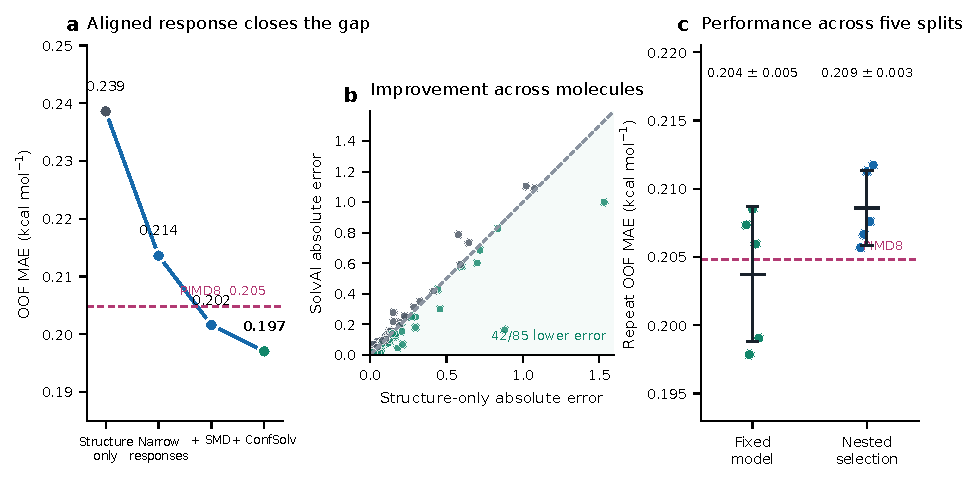
\includegraphics[width=\textwidth]{fig2_headline.pdf}
  \caption{\textbf{Aligned water response closes the gap to path-integral simulation.} \textbf{a}, Strict five-fold OOF progression for the same fixed endpoint protocol. The magenta line is the reconstructed ARROW/PIMD8 MAE on the same 85 solutes. \textbf{b}, Paired molecule-level absolute error for the earlier structure-only model and SolvAI; points below the diagonal improve. Although 42 of 85 individual errors decrease, larger corrections produce the lower aggregate MAE. \textbf{c}, Complete OOF MAEs for five independent partitions with the response block fixed or selected inside nested validation. Points are independent split repeats; black bars show mean $\pm$ sample s.d.}
  \label{fig:headline}
\end{figure}

\section*{When physics transfers}

The gain was not a generic consequence of adding physical features. Compact ConfSolv response summaries transferred better than graph or feed-forward latent embeddings trained on the same source (Fig.~\ref{fig:transfer}a). Broader screens of force-field hierarchies, interaction energies, learned implicit response and three-dimensional representations also failed to improve the matched endpoint (Extended Data Fig.~3). These comparisons do not rank the underlying physical methods. They measure whether a physical quantity can itself be reconstructed from structure with enough precision to help hydration prediction.

Short PIMD2 calculations at coupling values $\lambda=0.1$, 0.5 and 0.9 provided a direct test of that condition. Structure-only response heads captured broad trends, but component MAEs ranged from 1.27 to 5.20 kcal mol$^{-1}$ (Fig.~\ref{fig:transfer}b). Adding the predicted response raised matched endpoint MAE from 0.196 to 0.201 kcal mol$^{-1}$; a classical--NQE--PIMD hierarchy reached 0.215 kcal mol$^{-1}$, and combining both reached 0.219 kcal mol$^{-1}$ (Fig.~\ref{fig:transfer}c). Direct integration of the predicted response curve gave 1.51 kcal mol$^{-1}$ (Extended Data Fig.~5).

The mechanistic conclusion is simple. Physical supervision helps only when the relevant response is learnable from the deployed input. SMD water response and conformer-distribution summaries were available across tens to hundreds of thousands of benchmark-disjoint structures and could be compressed into useful priors. Sparse high-fidelity response labels remained too difficult to infer at the precision required by the endpoint. PIMD2 and PIMD8 supervision were therefore evaluated but not retained.

\begin{figure}[t]
  \centering
  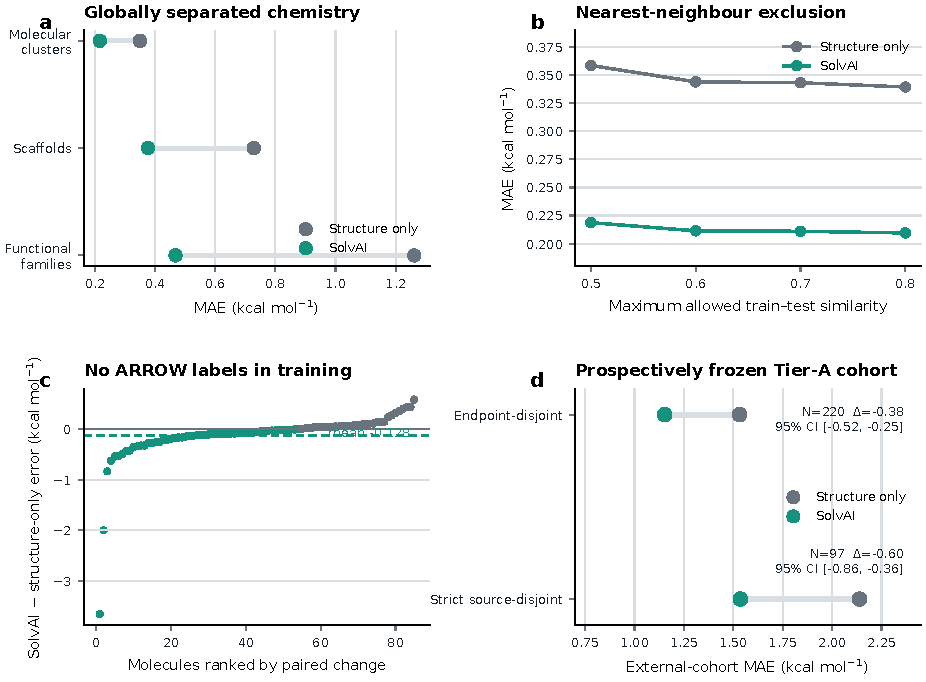
\includegraphics[width=\textwidth]{fig3_transfer.pdf}
  \caption{\textbf{Transfer depends on structure-to-response accuracy.} \textbf{a}, In a matched one-seed representation screen, six compact ConfSolv response summaries outperform graph and feed-forward latent coordinates from the same source. \textbf{b}, OOF error for structure-predicted PIMD2 total, electrostatic and van der Waals $\mathrm{d}H/\mathrm{d}\lambda$ responses. \textbf{c}, Downstream endpoint error for the matched baseline, predicted PIMD2 response, predicted fidelity hierarchy and their combination. Direct integration is reported separately because its error lies on a different scale. None of the PIMD-derived blocks is present in final SolvAI.}
  \label{fig:transfer}
\end{figure}

\section*{The present frontier}

The interpolation result does not remove the problem of chemical extrapolation. Holding out complete functional-group families gives an MAE of \FamilyMAE{} kcal mol$^{-1}$; scaffold holdout gives \ScaffoldMAE{} kcal mol$^{-1}$ (Fig.~\ref{fig:frontier}a and Extended Data Fig.~6). Random-OOF errors are largest for amides, aromatics, ethers, acids and alkanes, although several families contain only three to five solutes and should be read as diagnostic examples rather than population rankings (Fig.~\ref{fig:frontier}b). Molecule-bootstrap and paired-resampling results are reported in Extended Data Fig.~7.

The primary reference comprises only 85 molecules, and method development occurred in its context. The result is therefore a direct comparison on the molecular set used to establish ARROW/PIMD8 accuracy, not an across-dataset FreeSolv ranking. The complete method comparison, including the non-deployable simulation-assisted branch, appears in Extended Data Table~1 and Extended Data Fig.~4.

The response experiment points to a specific next dataset rather than a larger generic model. Approximately 250--500 protocol-matched molecules, with deliberate coverage of the five high-error families, should report full $\lambda$-resolved $\mathrm{d}H/\mathrm{d}\lambda$, electrostatic, polarization and dispersion/repulsion components, and paired classical and PIMD8 values (Fig.~\ref{fig:frontier}c). Such data would test whether high-fidelity response itself can become a reliable structure-derived prior.

SolvAI changes the computational role assigned to molecular simulation. A physical calculation need not be repeated for every prediction to remain useful. It can define transferable response coordinates, train structure surrogates and reveal exactly where structural inference breaks down. Rather than being invoked per query, expensive solvation physics can become reusable supervision for deployable molecular models.

\begin{figure}[t]
  \centering
  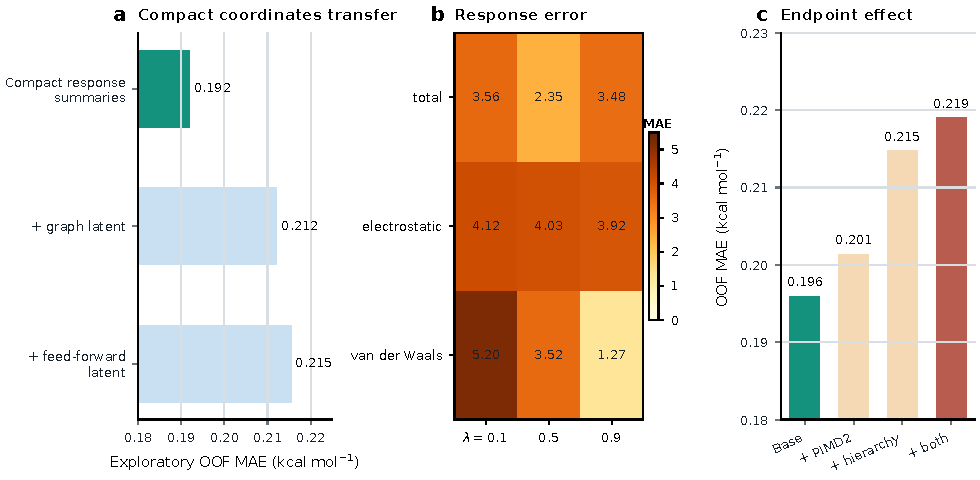
\includegraphics[width=\textwidth]{fig4_frontier.pdf}
  \caption{\textbf{Chemical extrapolation and response prediction define the frontier.} \textbf{a}, Random OOF, family-held-out and scaffold-held-out MAE for the fixed SolvAI stack; the dashed magenta line marks the PIMD8 reference. \textbf{b}, Molecule-level random-OOF absolute errors by chemical family. Vertical ticks give family means; sample sizes are displayed and five current high-error families are highlighted. \textbf{c}, The next informative training set is a protocol-matched, component-resolved alchemical response collection with paired classical and PIMD8 values, focused on underrepresented chemistry.}
  \label{fig:frontier}
\end{figure}

\FloatBarrier
\section*{Methods}

\subsection*{Reference set}

The primary evaluation uses the 85 neutral organic solutes reported in the ARROW hydration analysis at 298 K.\cite{arrow2022} The target is experimental hydration free energy in kcal mol$^{-1}$. One water condition was retained per molecular identity. The released table records canonical structure, source identifiers, experimental uncertainty where available, classical ARROW, PIMD4 and PIMD8 values, chemical-family annotation, scaffold and all validation assignments. The exact reconstructed PIMD8 MAE is \PIMDMAE{} kcal mol$^{-1}$; the original article reports approximately 0.20 kcal mol$^{-1}$.

\subsection*{Identity exclusion}

RDKit 2026.03.5\cite{rdkit2026} was used to parse each molecule and generate canonical isomeric SMILES and an InChIKey. External supervised sources were compared against the reference by canonical SMILES, full InChIKey and the 14-character connectivity block. Any connectivity match was removed before a teacher or endpoint model was fitted. For solvent-conditioned collections, the exclusion was applied across solvents. Invalid, disconnected, charged or unresolved rows were removed according to the frozen source manifests. A release audit independently repeats canonicalization and verifies zero retained overlap for every source used by SolvAI. Detailed source counts are given in Extended Data Fig.~2 and Supplementary Table~2.

\subsection*{Molecular representation}

The endpoint uses 2,265 deterministic structure features: a 2,048-bit radius-2 Morgan fingerprint and 217 RDKit two-dimensional descriptors. The frozen preprocessing replaces non-finite values using training-derived handling. No optimized three-dimensional conformer, trajectory or ARROW parameterization is required.

\subsection*{Response surrogates}

The 15 priors are generated by six frozen teacher artifacts (Supplementary Table~1). Two directed message-passing neural networks (D-MPNNs) predict the CombiSolv-QM COSMOtherm and MolSolv SMD(water) targets.\cite{chemprop2019} The former begins from a CHEMELEON foundation checkpoint and also receives RDKit descriptors; the latter begins from the same checkpoint and uses the molecular graph. Five Abraham targets and the OpenFF and GBn2 response pairs use extremely randomized trees.\cite{extratrees2006} Six selected ConfSolv targets use gradient-boosted trees. Corrected OpenFF and GBn2 coordinates are each the sum of a predicted physical value and a separately predicted experimental residual. The response vector contains only surrogate predictions at inference.

The final selected stack contains no PIMD-trained coordinate. PIMD2 response and PIMD8/classical hierarchy heads were trained only as predefined candidate ablations and were excluded after non-improving held-out results. PIMD8 is used in the paper as an independent high-fidelity reference.

\subsection*{Endpoint supervision}

The endpoint training pool combines 1,280 benchmark-disjoint public experimental hydration labels with the reference molecules available in each outer-training fold. The public set comprises 1,147 rows from a connectivity-resolved FreeSolv/CombiSolv-Exp merge and 133 SoluteML dGsolvDB3 rows supported by at least two source measurements.\cite{freesolv2017,combisolvexp2022,soluteml2022} External rows have sample weight one and outer-training reference rows weight three. The public deployment artifact was refitted after evaluation on the 1,280 external labels and all 85 reference labels; none of its refit predictions is used as held-out evidence.

The hydration model is an ensemble of three \texttt{ExtraTreesRegressor} instances with 360 trees, maximum feature fraction 0.7, minimum leaf size 2 and seeds 11, 29 and 47. It receives the 2,265 structure features and 15 predicted response priors. Ensemble predictions are averaged. The complete source, teacher and endpoint specifications are provided in Supplementary Methods.

\subsection*{Evaluation}

Random OOF evaluation uses five frozen molecule-level folds. For every reference molecule, the endpoint excludes its experimental label. Externally trained teachers never contain its connectivity. The fixed-block result evaluates the response representation selected during the completed campaign; the nested procedure selects among narrow response, SMD and ConfSolv blocks using inner-OOF predictions from each outer-training partition. Five independent complete five-fold repetitions use seeds 314159, 271828, 161803, 141421 and 173205. Grouped folds hold out functional-group families; scaffold folds use the frozen scaffold grouping. Exact assignments are provided as Supplementary Data~3.

\subsection*{Statistics}

MAE is the primary endpoint; RMSE is retained in the machine-readable metric file. Percentile intervals were calculated from 100,000 molecule-level bootstrap resamples with seed 20260827. Paired comparisons resampled molecule-wise error differences, preserving predictions on the same solute. Repeated-split variation is reported as mean $\pm$ sample s.d. across five complete partitions. No inferential test was used to declare a 0.20-kcal mol$^{-1}$ threshold crossing.

\subsection*{Lambda-response test}

Short, training-only PIMD2 calculations were available at $\lambda=0.1$, 0.5 and 0.9 for 72, 74 and 73 molecules, respectively; 72 had complete three-point curves. Each run used 5 ps at one coupling state and was interpreted as a response fingerprint, not a converged free energy. Total, Coulomb and van der Waals $\mathrm{d}H/\mathrm{d}\lambda$ targets were predicted with all held-out molecule response labels excluded. The frozen experiment compared the matched endpoint alone, the predicted response, a classical--NQE--PIMD hierarchy, their combination, and affine-calibrated integration. Full protocols and results appear in Supplementary Methods and Extended Data Fig.~5.

\subsection*{Runtime and release audit}

The packaged artifact was measured from SMILES input to hydration output on an Intel Core i7-4930K CPU; the installed RTX 3090 was not used. After one warm-up, five single-molecule calls gave a median of 17.522 s and p95 of 17.627 s. Three batches of 32 molecules gave a median of 17.911 s, or 0.560 s per molecule. The current implementation starts separate response-model processes, so single-query latency is an engineering property rather than a minimum scientific cost. Published ARROW/PIMD8 timings used an RTX 2080 Ti and 15 one-nanosecond windows, corresponding to 240--270 serial GPU-hours;\cite{arrow2022} because hardware differs, we report this only as a total-work context, not a same-device speed benchmark.

The release audit verifies artifact SHA-256 values, runs ethanol and benzene smoke predictions from SMILES, searches the runtime schema for prohibited target and simulation fields, and reruns the connectivity exclusions. The repository contains exact environments, prediction tables, metric reconstruction, figures and manuscript source.

\section*{Data availability}

The reference table, held-out predictions, validation assignments, derived metrics and redistributable processed teacher tables are included in the SolvAI repository. Source URLs, versions, licences, checksums, filtering and reproduction commands are recorded in \path{repro/DATA_PROVENANCE.md}. Third-party data without explicit redistribution terms must be obtained from their original provider.

\section*{Code availability}

Inference, audits, frozen metric reconstruction, figure generation and manuscript source are available at \url{https://github.com/Scientific-Computing-Lab/SolvAI}. The released command accepts a SMILES string and starts no simulation software.

\bibliographystyle{unsrtnat}
\bibliography{references}

\clearpage
\section*{Extended Data legends}

\noindent\textbf{Extended Data Fig. 1 | Molecular predictions and residual diagnostics.} \textbf{a}, Experimental and strict OOF SolvAI hydration free energies; the diagonal denotes equality. \textbf{b}, Signed residual against experimental hydration free energy. \textbf{c}, Absolute errors for the previous structure-only model and SolvAI, ordered by SolvAI error. The logarithmic scale exposes small and large residuals simultaneously.

\medskip
\noindent\textbf{Extended Data Fig. 2 | Source-specific provenance and identity exclusion.} Each row retains its native source unit. FreeSolv overlap describes the identity relationship of the reference set and does not define an external test. MolSolv and ConfSolv rows report benchmark matches removed before teacher fitting and the final source-specific training counts. Unlike identities, calculations and conformer records are not placed on a common quantitative axis.

\medskip
\noindent\textbf{Extended Data Fig. 3 | Alternative routes to physics-informed hydration prediction.} Frozen OOF screens of candidate physical supervision and representations. Values follow their documented matched regimes and compare transfer utility rather than the intrinsic accuracy of the source calculation. The matched one-seed base is the reference for these screens. Full experiment definitions are provided as Supplementary Data~1.

\medskip
\noindent\textbf{Extended Data Fig. 4 | Simulation-assisted accuracy--cost reference.} Oracle and nested learned routing under the original random-OOF analysis. These policies require PIMD8 for selected test molecules and are not part of SolvAI or any structure-only headline result. The panel is retained as a non-deployable scientific reference.

\medskip
\noindent\textbf{Extended Data Fig. 5 | Multi-$\lambda$ response distillation.} \textbf{a}, Structure-to-response MAE for total, electrostatic and van der Waals components at three coupling values. \textbf{b}, Matched endpoint error for the baseline and three predicted-physics additions. \textbf{c}, Direct integration of the predicted response, shown on its own scale. Prediction error in the physical response, rather than endpoint capacity, is the limiting step.

\medskip
\noindent\textbf{Extended Data Fig. 6 | Chemical extrapolation.} \textbf{a}, Random, family and scaffold holdout MAE. \textbf{b}, Random-OOF and family-holdout MAE for each annotated family; sample sizes are shown. \textbf{c}, Scaffold-holdout absolute error across the hydration range. Small family groups are diagnostic and are not interpreted as precise population rankings.

\medskip
\noindent\textbf{Extended Data Fig. 7 | Bootstrap and paired uncertainty.} \textbf{a}, Fixed and nested OOF point estimates with molecule-bootstrap 95\% intervals. \textbf{b}, Paired molecule-bootstrap MAE differences relative to the previous structure-only model and PIMD8; zero denotes equal point performance.

\medskip
\noindent\textbf{Extended Data Table 1 | Final model and evaluation comparison.} Mean absolute errors are in kcal mol$^{-1}$. Dashes denote evaluations not defined for that frozen artifact. Only rows with no simulation at inference satisfy the SolvAI deployment definition.

\end{document}
